\documentclass[UTF8]{article}
\usepackage{cite}
\usepackage[unicode,pdftex]{hyperref}
\usepackage{enumerate}
% \usepackage{geometry}
\usepackage{setspace}
\usepackage{pslatex} 
\usepackage{fancyhdr}
\usepackage{float}
\usepackage{amsmath}
\usepackage{titling}
\usepackage{indentfirst}
\usepackage{graphicx}
\usepackage{wrapfig}
\usepackage{amsmath}
\usepackage{xstring}
\usepackage{multirow}
\usepackage{amsmath}
\usepackage{verbatim}
\usepackage{multirow}
\usepackage{array}
\usepackage{diagbox}[2011/11/22]
\usepackage{mathrsfs}
\usepackage{amsfonts}
\usepackage{mathtools}
\usepackage{multirow}
\usepackage{xcolor}
\usepackage{amssymb}

\usepackage{tikz}
\usetikzlibrary{fit, calc}
\pagestyle{empty} 



% \geometry{left=2.5cm, right=2.5cm, top=1.4cm, bottom=2.4cm}
\usepackage[a4paper,top=3cm,bottom=2cm,left=3cm,right=3cm,marginparwidth=1in, margin=1in]{geometry}
% \usepackage[margin=1in]{geometry}
\title{Assignment 1 Report}
\author{Chenqiu Zhao(zhao.chenqiu@ualberta.ca)}
\date{}


\newcommand{\reffig}[1]{Fig. \ref{#1}}
\newcommand{\refsec}[1]{Section \ref{#1}}
% \newcommand{\refeq}[1]{Eq. \ref{#1}}
\newcommand{\reftab}[1]{Table \ref{#1}}
\newcommand{\tabincell}[2]{\begin{tabular}{@{}#1@{}}#2\end{tabular}}


\renewcommand{\tabincell}[2]{\begin{tabular}{@{}#1@{}}#2\end{tabular}}


\fancyhead{}
\lhead{\scriptsize Chenqiu Zhao}
\rhead{\scriptsize research Proposal}

\renewcommand{\headrulewidth}{0pt}
\renewcommand{\normalsize}{\fontsize{12pt}{\baselineskip}\selectfont}


\newcommand{\chronoperiode}[7]{
  \pgfmathsetmacro{\first}{(#2 - 2018)*12 + #3 - .9} % beginig of the peropd
  \pgfmathsetmacro{\last}{(#4 - 2018)*12 + #5 - 1.1} % end of the period
  \pgfmathsetmacro{\middle}{(\first+\last)/2} % position of the country name
  \fill[#7] (\first,#6-1) rectangle (\last,#6) (\middle,#6-.5) node[white, font=\sf]{#1};
}

\definecolor{level1}{RGB}{200,10,20}
\definecolor{brightube}{rgb}{0.82, 0.62, 0.91}
\definecolor{fuchsia}{rgb}{1.0, 0.0, 1.0}
\definecolor{heliotrope}{rgb}{0.87, 0.45, 1.0}



\begin{document}
\maketitle
%\vspace{-90pt}






% \section*{Abstract}
% % 以前方法都是用
% Previous approaches to background subtraction typically proposed artificial model to approximate the distribution of pixels' observations.
% % 为什么distribution 可以用
% In this proposal, we focus on learning the distribution of observations automatically instead of devising sophisticated model.
% %
% In particular,
% the deep learning network is naturally selected to learn the distribution,
% due to it is excellent learning ability.
% %
% Moreover,
% distribution itself has wide range of applications as well.
% %
% Therefore, the distribution learning can not only be used in the background subtraction but also in many other fields.
% %
% Hence,
% just like the hierarchical features learned by deep learning network,
% we assume that there is high level representation of distribution which should work better than all these existed statistic techniques related to distribution,
% and we named this level representation as "Deep Distribution", which is the final target of this proposal.
% %
% 

% 以前distribution的确定是什么

% 你打算怎么做

% 具体怎么做

% 可以做成个什么样子


\section*{Question 1}
% \subsection*{Data preparation:}
\begin{wrapfigure}{l}{0.3\textwidth}
%  \vspace{-15pt}    % 对应高度1
  \includegraphics[width=0.3\textwidth]{../imgs/showim.png}
    \label{fig1}
%  \vspace{-15pt}    % 对应高度2
%  \vspace{-15pt}    % 对应高度3
\end{wrapfigure}

There are 113 images in Microscopy dataset, which is download from the link provided in the assignment document.
%
In particular,
50 images are labelled as positive and 63 images are classified as negative.
%
Positive images and negative images are randomly split into 3 parts, training(70\%), validation(20\%) and test(10\%) sets respectively,
to guarantee that the proportion of positive and negative samples keep invariant in these three sets.
%
For a particular image,
patches with size of $60 \times 60$ are extracted,
in which the position of patches are randomly generated.
%
With the consideration of memory cost, 200 patches are extracted from one image, as shown in the left figure.
%
Totally, 15800 patches are utilized for training.

\begin{wraptable}{r}{0.55\textwidth}
\label{tab_net}				% LABEL: tab7
% \scriptsize
\footnotesize
\centering
 \begin{tabular}{|l|l|l|l|}
\hline
     Type                   & Filters   & Layer size   & Data size     \\
\hline
     Input                  &           &                       &   $60\times60\times3$   \\
     Convolution            & 20        & $10\times10\times3$   &   $51\times51\times20$  \\
     Rectified linear unit  &           &                       &   $51\times51\times20$  \\
     Max pooling            &           & $2 \times 2$ with stride of 2          &   $25\times25\times20$  \\
     Convolution            & 50        & $10\times10\times20$  &   $16\times16\times50$  \\
     Rectified linear unit  &           &                       &   $16\times16\times50$  \\
     Max pooling            &           & $2 \times 2$ with stride of 2         &   $8\times8\times50$   \\
     Convolution            & 500       & $8\times8\times50$    &   $1\times1\times500$  \\
     Rectified linear unit  &           &                       &   $1\times1\times500$  \\
     Convolution            & 2       & $1\times1\times500$     &   $1\times1\times2$   \\
     \text{Softmax}         &           &                       &                         \\
\hline
\end{tabular}
\end{wraptable}
Since, the assignment is a typical classification problem,
the network architecture is devised as a classification network, which is similar to LeNet.
%
The comprehensive details of the network architecture is shown the in the right table.
%
During training, 20 epochs are set as the maximum and $0.001$ is used as the learning rate.
%
It should be noted that our program is ran on a remote server instead of a local PC,
so we extract the training information and draw the plots by ourself.
%
The plots of training loss, validation loss, training accuracy and validation accuracy
are shown as follows:
\begin{figure*}[htbp]	% FIGURE: figure/fig1 
\centering
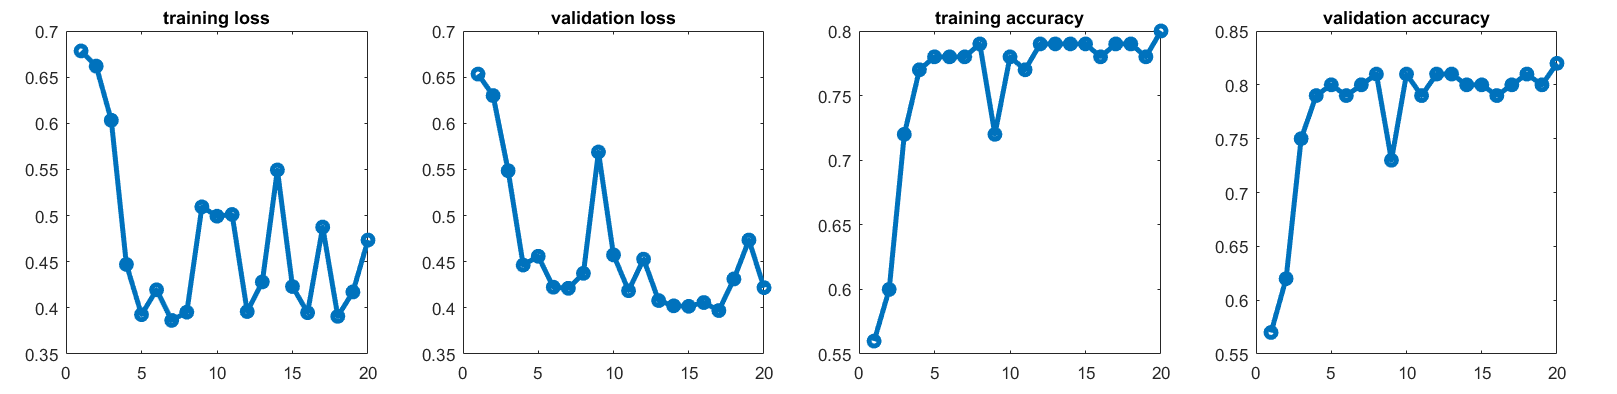
\includegraphics[width=\textwidth]{../imgs/loss.png}
\label{fig_bay}
\end{figure*}

After training,
the test set is utilized for evaluating the proposed network.
%
There are 11 images in the test set.
%
In particular, 5 images are labelled as positive and 6 images are labelled as negative.
%
During testing,
8 images are classified correctly,
the classification accuracy is $\frac{8}{11} = 0.7273$.
%
However,
in a real application,
the significance of positive and negative samples are different.
%
In order to propose a fair and comprehensie evaluation of the proposed network,
$Re$, $Pr$ and $Fm$ metrics are utilized for evaluation.
%
For the completeness of this report,
the definition of these metrics are briefly introduced.
Re and Pr are measures of completeness and accurateness, respectively. Fm is a combination of Re and Pr. These metrics are defined as follows:
\begin{displaymath}
    \begin{aligned}
        Re = \frac{TP}{TP + FN},
        Pr = \frac{TP}{TP + FP},
        Fm = \frac{2 \times Pr \times Re}{Pr + Re}
    \end{aligned},
\end{displaymath}
where TP and FP are True Positive and False Positive. True denotes that the result of this classification is correct, while False means otherwise.
Thus, TP means that the result of the detection is positive as well as being the groundtruth.

Moreover,
since the training set and test set are randomly split,
it is possible that the evaluation results are different for different repeating experiments.
%
In order to propose a fair evaluation,
we repeat the experiment 10 times, and the average performance is proposed as the final performance of the proposed network.
%
The results is shown as follows:
\begin{table*}[htbp]				% TABLE
    \small
\label{tab_bay}
\centering
%     \begin{tabular}{|l|c|c@{ }c@{ }c@{ }c@{ }c@{ }c@{ }c@{ }c@{ }c@{ }c@{ }|c|}
     \begin{tabular}{|l|c|cccccccccc|c|}

\hline
        \multicolumn{2}{|c}{Repeating Experiments }  & 1 & 2  & 3  & 4  & 5  & 6  & 7  & 8  & 9  & \multicolumn{1}{c@{ }}{10 } &  Average \\
\hline
        \multirow{3}{*}{ \tabincell{l}{  Single \\ Resolution }  }        & Re   & 0.8  & 0.6    & 1.0 & 0.6    & 0.8    & 1.0    & 0.8    & 0.8 & 1.0    & 0.8    & 0.8190 \\
        \cline{2-2}                                                                                                                                                                  
                                                                            & Pr   & 1.0  & 1.0    & 1.0 & 1.0    & 0.667 & 0.833 & 1.0    & 0.8 & 0.833 & 1.0    & 0.9001 \\
        \cline{2-2}                                                                                                                                                                  
                                                                            & Fm   & 0.89 & 0.749 & 1.0 & 0.749 & 0.727 & 0.909 & 0.889 & 0.8 & 0.909 & 0.889 & 0.8513 \\
         \hline
\end{tabular}
\end{table*}

\section*{Question 2}
\begin{wrapfigure}{l}{0.5\textwidth}
%  \vspace{-15pt}    % 对应高度1
  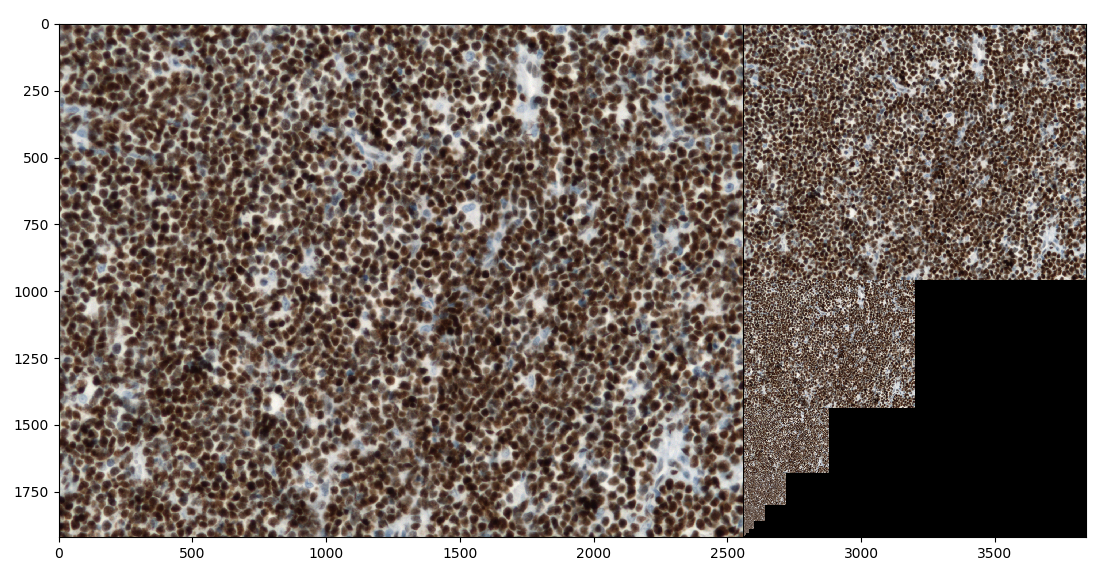
\includegraphics[width=0.5\textwidth]{../imgs/pymid.png}
    \label{fig1}
%  \vspace{-15pt}    % 对应高度2
%  \vspace{-15pt}    % 对应高度3
\end{wrapfigure}
The Gaussian pyramid construction of one microscopy image is demonstrated on the left figure.
%
Patches captured from images with frist three scales are directly combined to input into the network.
%
In particular,
the left-top positions of corresponding patches are keep invariant.
%
After combiniation, 
the size of patches becomes $60 \times 60 \times 9$.
%
In order to input these patches into the network,
we simply increase the channel of kernels in the first layer of network to 9,
the size of kernels in the first layer of network thus becomes $10 \times 10 \times 9$.
%
The network is trained by the same parameters with the single resolution experiments.
%
The plots of training loss, validation loss, training accuracy and validation accuracy
are shown as follows:
\begin{figure*}[htbp]	% FIGURE: figure/fig1 
\centering
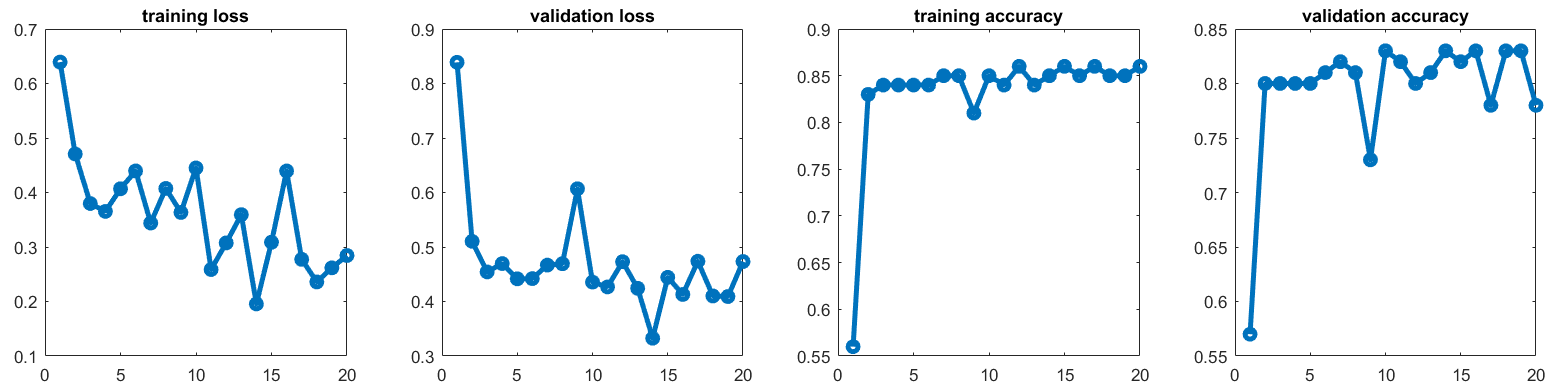
\includegraphics[width=\textwidth]{../imgs/mulloss.png}
%    \caption{none of these techniques are used in our previous DPDL \cite{2018_ICME_8486510} model in the last row. }
\label{fig_bay}
\end{figure*}
\begin{table*}[htbp]				% TABLE
    \small
\label{tab_bay}
\centering
%     \begin{tabular}{|l|c|c@{ }c@{ }c@{ }c@{ }c@{ }c@{ }c@{ }c@{ }c@{ }c@{ }|c|}
     \begin{tabular}{|l|c|cccccccccc|c|}

\hline
        \multicolumn{2}{|c}{Repeating Experiments }  & 1 & 2  & 3  & 4  & 5  & 6  & 7  & 8  & 9  & \multicolumn{1}{c@{ }}{10 } &  Average \\
\hline
        \multirow{3}{*}{ \tabincell{l}{  Single \\ Resolution }  }        & Re   & 0.8  & 0.6    & 1.0 & 0.6    & 0.8    & 1.0    & 0.8    & 0.8 & 1.0    & 0.8    & 0.8190 \\
        \cline{2-2}                                                                                                                                                                  
                                                                            & Pr   & 1.0  & 1.0    & 1.0 & 1.0    & 0.667 & 0.833 & 1.0    & 0.8 & 0.833 & 1.0    & 0.9001 \\
        \cline{2-2}                                                                                                                                                                  
                                                                            & Fm   & 0.89 & 0.749 & 1.0 & 0.749 & 0.727 & 0.909 & 0.889 & 0.8 & 0.909 & 0.889 & 0.8513 \\
         \hline
         \multirow{3}{*}{ \tabincell{l}{  Multiple \\ Resolutions }  }       & Re   & 0.8  & 0.8    & 1.0   & 1.0    & 0.8   & 0.8   & 0.8    & 1.0 & 1.0   & 1.0    & \textbf{0.9000} \\
        \cline{2-2}                                                                                                                                                                  
                                                                            & Pr   & 1.0  & 1.0    & 0.833 & 1.0    & 0.8   & 0.8   & 0.8    & 1.0 & 1.0   & 1.0    & \textbf{0.9233} \\
        \cline{2-2}                                                                                                                                                                  
                                                                            & Fm   & 0.89 & 0.89   & 0.896 & 1.0    & 0.8   & 0.8   & 0.8    & 1.0 & 1.0   & 1.0    & \textbf{0.9076} \\
         \hline
\end{tabular}
\end{table*}

Similar with the evaluation experiment proposed in last section,
the evaluation of network with multiple resolutions input is also repeated for 10 times.
%
The comparison between the network with single resolution input and multiple resolutions input is shown in the above table.
%
All the source codes and running results are available online \url{https://github.com/zhaochenqiu/courses/tree/master/CMPUT617/Assignment1/program}.

\newpage

\section*{Question 3}
\begin{wrapfigure}{l}{0.5\textwidth}
  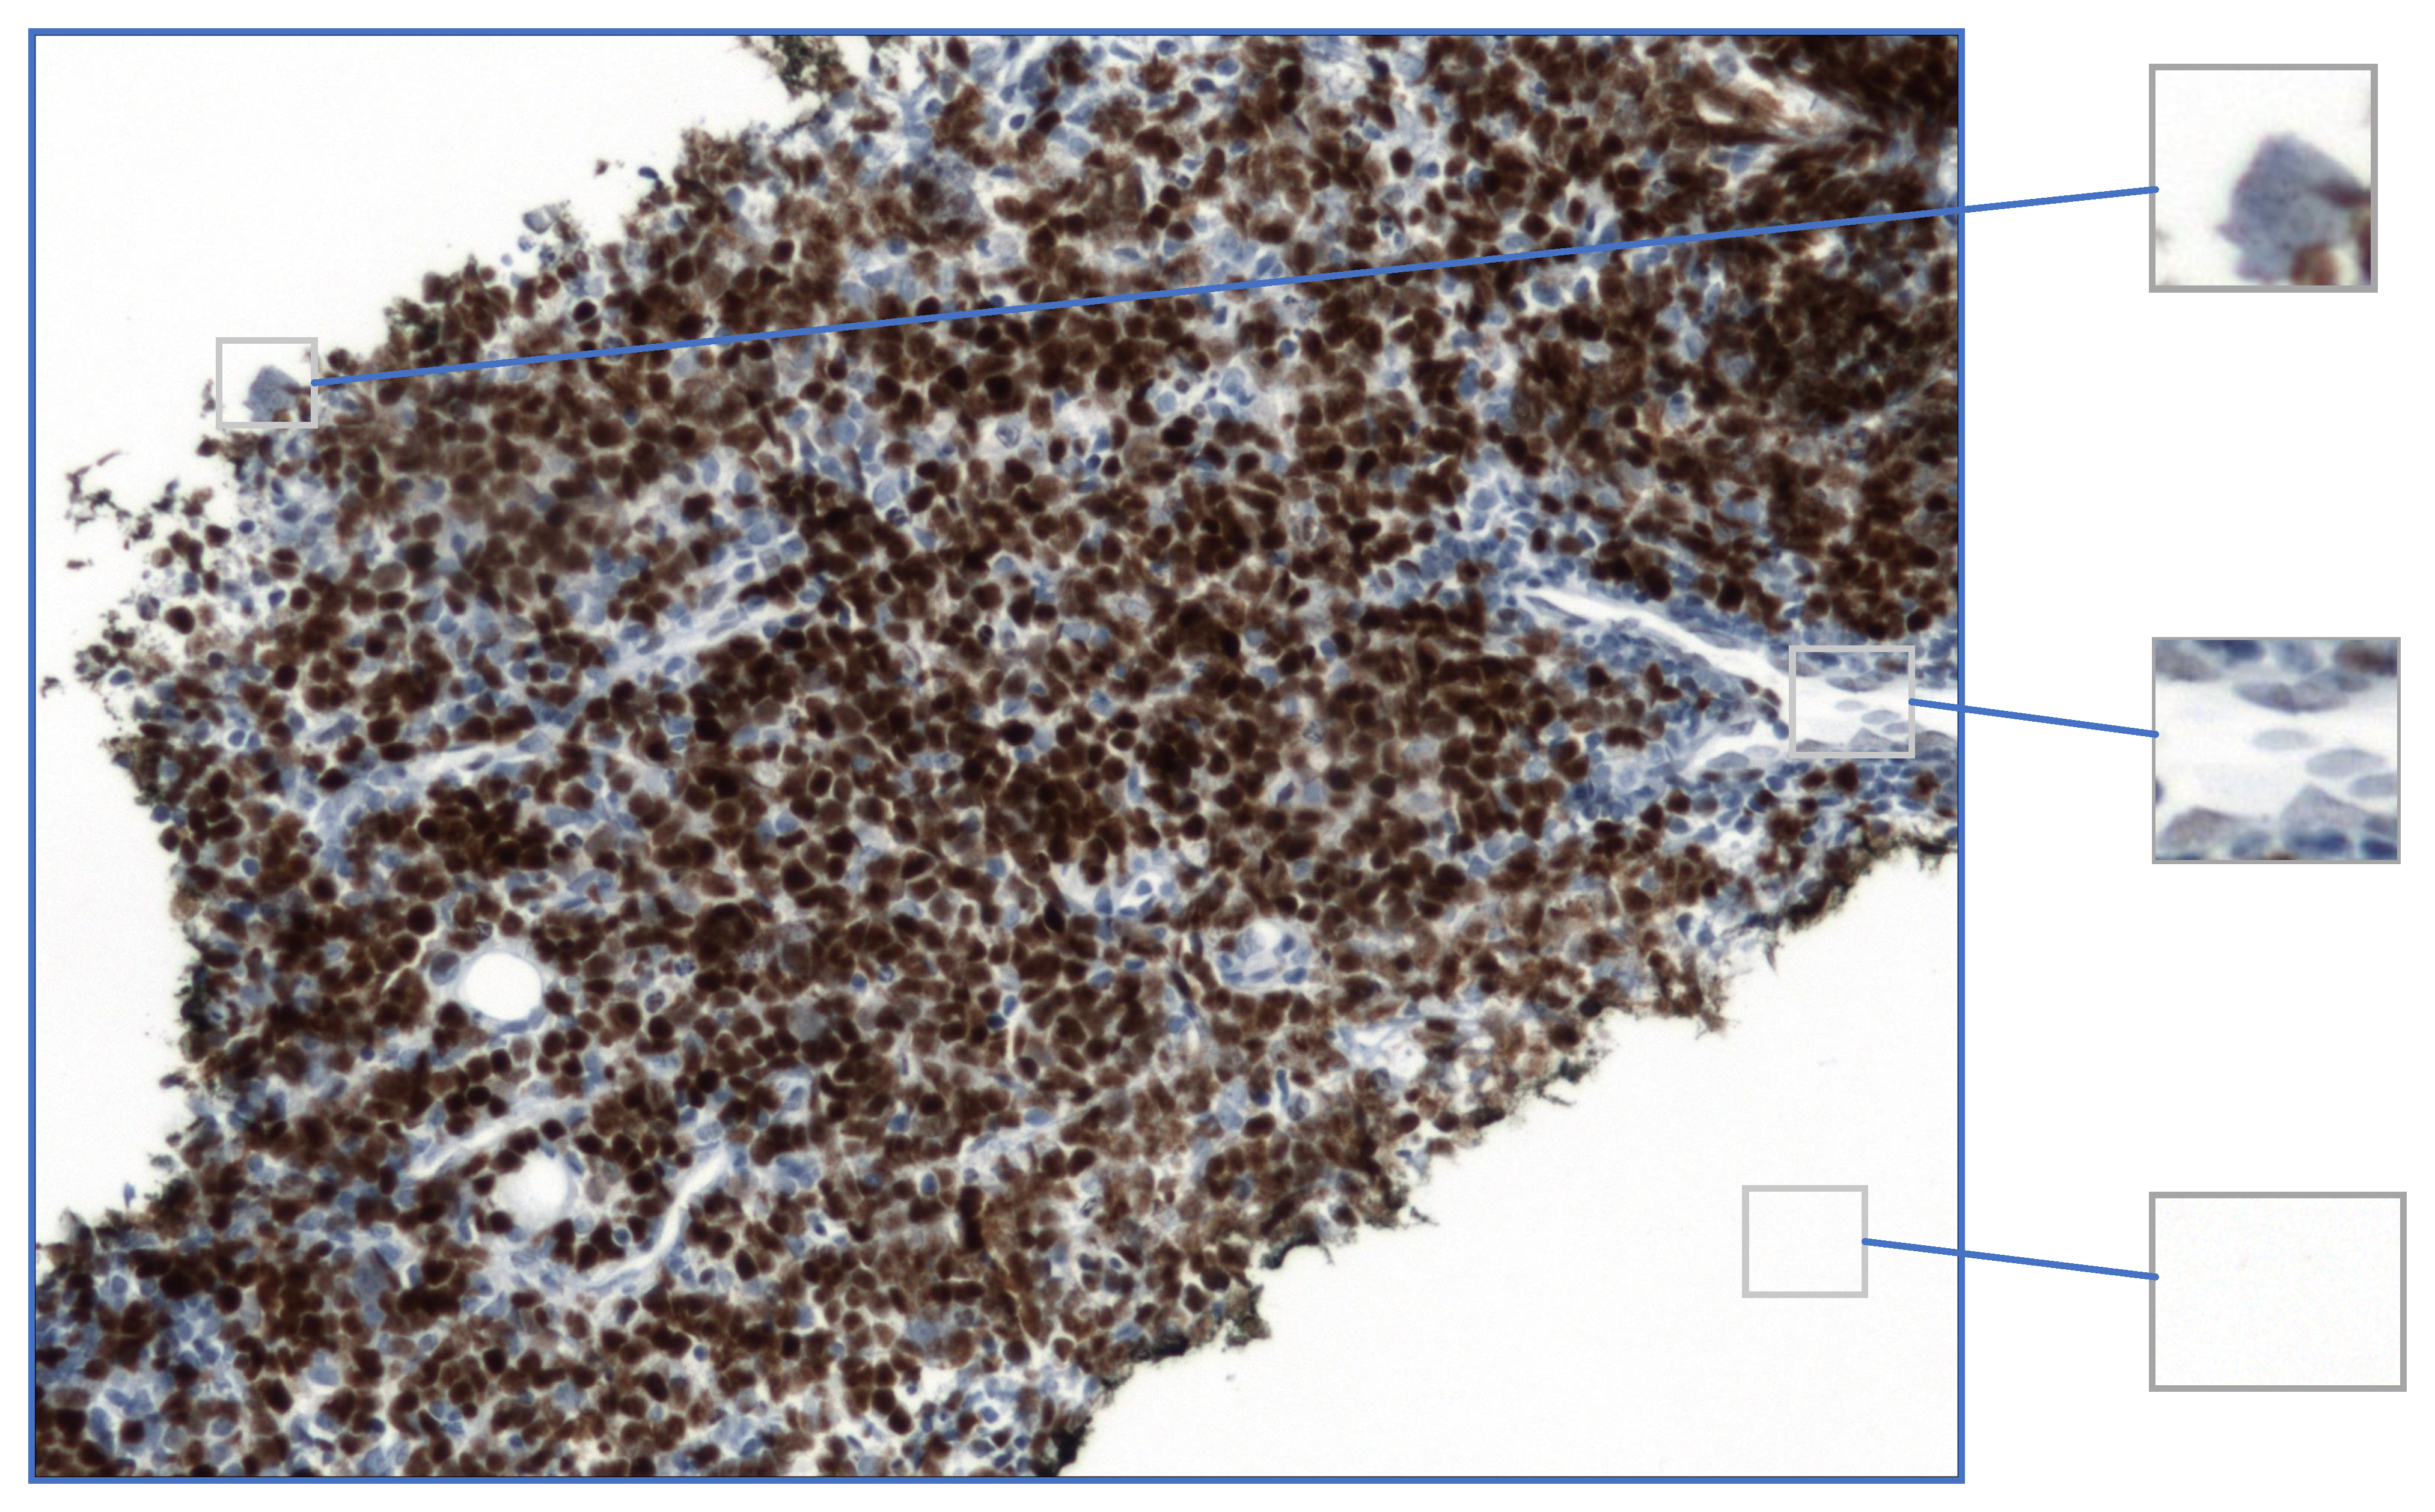
\includegraphics[width=0.5\textwidth]{../imgs/test.pdf}
    \label{fig1}
\end{wrapfigure}
In my opinion,
the generation of training data is the main challenge of applying deep learning to microscopy over the traditional method.
%
Since the resolution of microscopy image is too large to be input into convolutional neural directly,
patches captured from images are utilized as a compromise to be fed into the network for training.
%
Moreover, the size of patches has significant influence on the performance of network,
since there may be no completed cell in a patch when the size is small,
while the patches with large size will cost a lot of memory.
Hence, 
because the labels of patches are decided according to the name of microscopy image,
it is possible that some patches without any cells are labeled as positive like patches shown in the left figure.
%
These patches play the role of distraction during training network.
%
In contrast, since the method proposed in the paper \cite{bigras2018new} is a dimensionless method,
with the utilization coefficient of variation, which is a dimensionless feature.
%
The cells are detected by local maximum algorithms, 
and there is no need to consider the generation of training data.

Of course, there are also advantages for applying deep learning to microscopy images classification.
%
As shown in the table above, 
the performance of deep learning is one of the biggest advantages.
%
Unlike previous traditional methods,
the hierarchy architecture of deep learning network makes the model has the ability to learn 
high-level features which is better than these manual features.
%
Moreover,
the deep learning network can automatically learn the features which are suitable for the applications,
such as microscopy image classification.
%
From this perceptive,
the generality of a deep learning network is better than the traditional method.

Finally,
I'd like to discuss another disadvantage of applying deep learning network to microscopy image classification.
%
As we can see,
there is not very high similarity  between the visual patterns in different microscopy images,
since it seems that the size and the positions of cells include randomness.
%
    In this condition,
it is possible that the patterns in the test set may never appear in training set,
and the performance of deep learning network is not promising.
%
Personally,
I think it is the main reason that the performance of the proposed network varies during repeating experiments.


% In addition,
% it is possible that some patches didn't include any cell but still labelled as positive,
% since we label patches accoridng to the image, but the image did not fill with cells.
% such as the shown in XXX, the patches did not incldue any cell.
% Actually,
% such condition usually happend in the training data.
% I personelly think that it is the main reason why the loss of network is far away from 0,
% and it is also the reason that why the testing accuracy only around 75\%.
% In contast,
% the method utilized the local maximunm, which has much better ability to find the cell.
% 
% Finally,
% i would like to dicuss the weekness of convolutional neural network.
% %
% One of the most import weekness of neural networkm is that the network is not converange.
% %
% It may produce high confience when the input is not a cell image.
% %
% Inspired by \cite{nguyen2015deep}.
% %
% Also, the network requires that the training data mush include all potential variable,
% which makes the the extension of network is pool.
% %
% Although there is a incredamental learning,
% but it still requires the data
% 



\small
\bibliographystyle{unsrt}
% \bibliographystyle{plain}
\bibliography{ref.bib}  




\end{document}
